% Created 2023-08-02 Wed 16:43
% Intended LaTeX compiler: pdflatex
\documentclass[11pt]{article}
\usepackage[utf8]{inputenc}
\usepackage[T1]{fontenc}
\usepackage{graphicx}
\usepackage{longtable}
\usepackage{wrapfig}
\usepackage{rotating}
\usepackage[normalem]{ulem}
\usepackage{amsmath}
\usepackage{amssymb}
\usepackage{capt-of}
\usepackage{hyperref}
\usepackage{listings}
\usepackage{color}
\usepackage{amsmath}
\usepackage{array}
\usepackage[T1]{fontenc}
\usepackage{natbib}
\author{Anders Munch}
\date{\today}
\title{statelearner sim results}
\begin{document}

\maketitle

\section{IPCW with KM can fail}
\label{sec:org87e728e}
\begin{center}
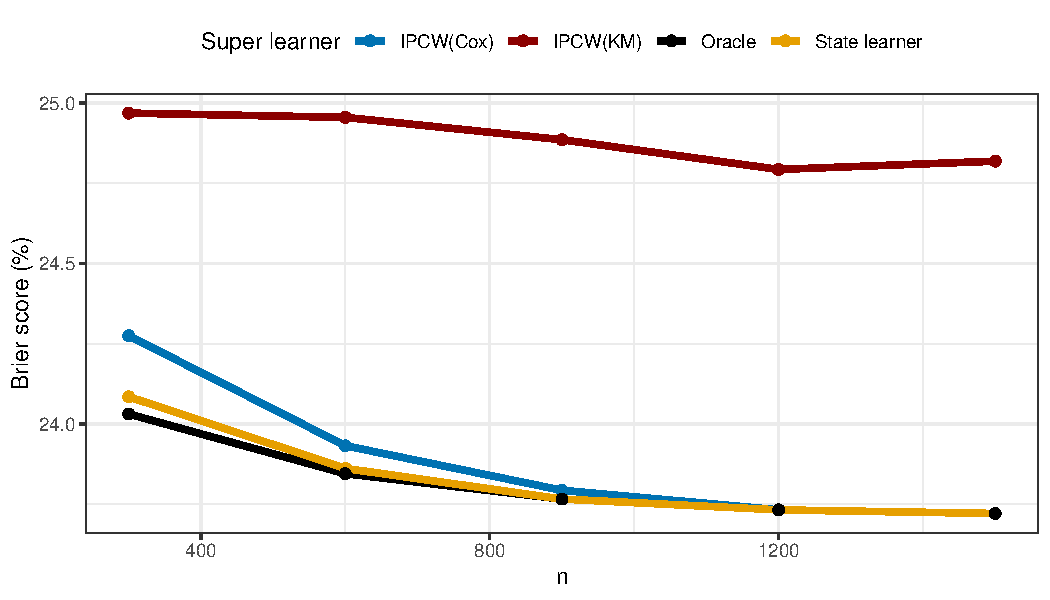
\includegraphics[width=.9\linewidth]{ipcw-fail.pdf}
\end{center}


\section{Zelefski data}
\label{sec:orgffdb325}
\subsection{Larger sim study with rf and glmnet including IPCW(cox)}
\label{sec:org14cd83f}

\begin{center}
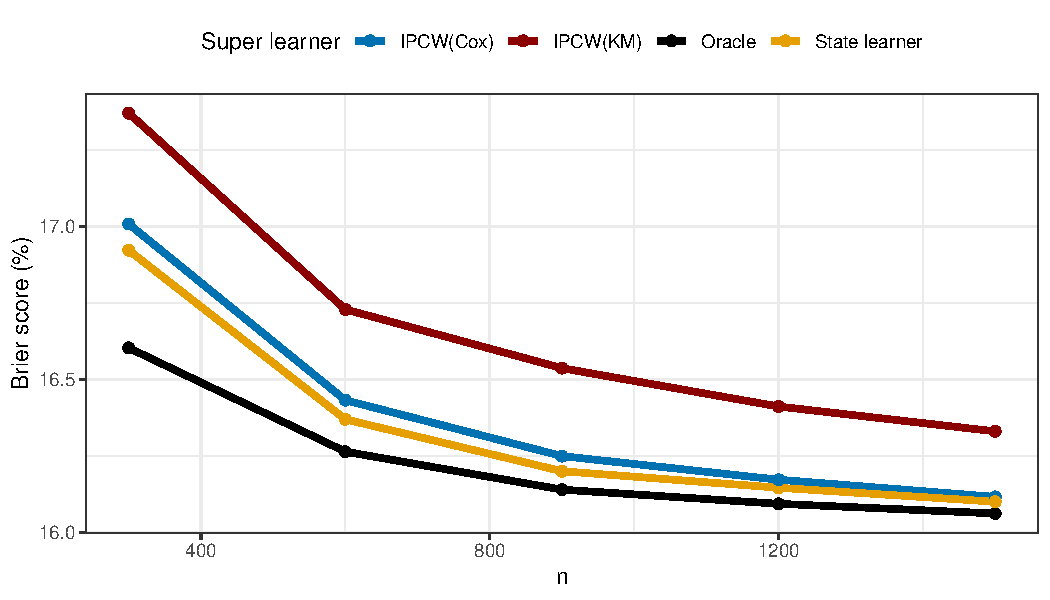
\includegraphics[width=.9\linewidth]{zelefski-sim.pdf}
\end{center}

Oracle risk for all models.

\begin{center}
\includegraphics[width=.9\linewidth]{/tmp/babel-P8DnIK/figure-FTlXlU.pdf}
\end{center}
\end{document}